%Authors guidlines: http://royalsocietypublishing.org/instructions-authors
% 2500 words max (includes the title page, abstract, references, acknowledgements and figure/table legends)
% current version is around 3700. I think a big cut down can be done on the references.
% We allow a maximum of 4 displays, only 2 of which can be figures.

\documentclass[12pt,letterpaper]{article}


%Packages
\usepackage{pdflscape}
%\usepackage{fixltx2e}
\usepackage{textcomp}
\usepackage{fullpage}
\usepackage{float}
\usepackage{latexsym}
\usepackage{url}
\usepackage{epsfig}
\usepackage{graphicx}
\usepackage{amssymb}
\usepackage{amsmath}
\usepackage{bm}
\usepackage{array}
%\usepackage{mhchem}
\usepackage{ifthen}
\usepackage{caption}
\usepackage{hyperref}
\usepackage{amsthm}
\usepackage{amstext}
\usepackage{enumerate}
\usepackage[osf]{mathpazo}
\usepackage{dcolumn}
\usepackage{lineno}
\usepackage{longtable}

\pagenumbering{arabic}

\newcolumntype{L}[1]{>{\raggedright\let\newline\\\arraybackslash\hspace{0pt}}m{#1}}
\newcolumntype{C}[1]{>{\centering\let\newline\\\arraybackslash\hspace{0pt}}m{#1}}
\newcolumntype{R}[1]{>{\raggedleft\let\newline\\\arraybackslash\hspace{0pt}}m{#1}}

%Pagination style and stuff % NC: Note that these are all syst biol specific.
\linespread{2}
\raggedright
\setlength{\parindent}{0.5in}
\setcounter{secnumdepth}{0} 
\renewcommand{\section}[1]{%
\bigskip
\begin{center}
\begin{Large}
\normalfont\scshape #1
\medskip
\end{Large}
\end{center}}
\renewcommand{\subsection}[1]{%
\bigskip
\begin{center}
\begin{large}
\normalfont\itshape #1
\end{large}
\end{center}}
\renewcommand{\subsubsection}[1]{%
\vspace{2ex}
\noindent
\textit{#1.}---}
\renewcommand{\tableofcontents}{}
%\bibpunct{(}{)}{;}{a}{}{,}

%---------------------------------------------
%
%       START
%
%---------------------------------------------

\begin{document}

%Running head
\begin{flushright}
Version dated: \today
\end{flushright}

\bigskip
\medskip
\begin{center}

\noindent{\Large \bf The Effect of Vulture Declines on Nutrient Spread} 

\bigskip

\noindent {\normalsize \sc Adam Kane$^1$$^,$$^*$ and Andrew Jackson$^2$}\\

 1. University College Cork, Cooperage Building, School of Biological Earth and Environmental Sciences, Cork, Ireland. \\
 2. Trinity College Dublin, Department of Zoology, School of Natural Sciences, Dublin 2, Ireland; Trinity Centre for Biodiversity Research, Trinity College Dublin, Dublin 2, Ireland.
\end{center}
\medskip
\noindent{*\bf Corresponding author.} \textit{adam.kane@ucc.ie}\\  
\vspace{1in}

%Line numbering
\modulolinenumbers[1]
\linenumbers

%---------------------------------------------
%
%       ABSTRACT
%
%---------------------------------------------
\newpage
\begin{abstract}
%\section{abstract} : Just put this here as it then separates this for the word count

\end{abstract}

\noindent Key words: vultures, nutrient transfer, ecosystem services, scavengers, hyenas\\


\vspace{1.5in}

%---------------------------------------------
%
%       INTRODUCTION
%
%---------------------------------------------
\newpage 
\section{Introduction}

% Animals provide a host of services that contribute to a functioning global ecosystem. 
% Notable among these is the ability to spread nutrients. 
Consider the diversity of animals that can end up feeding at the carcass of an elephant.
Here we have an incredibly dense and nutrient rich patch that ends up being distributed widely.
Scavengers also provide useful ecosystem services by acting as barriers to the spread of disease by quickly consuming rotting carcasses which have often died from illness \cite{ogada2012dropping}.
% "However, in general, vertebrate scavenging represents the widest dispersal of nutrients and energy from carcasses as vertebrate movement scales away to the broader landscape" \cite{benbow2015introduction}
%"This dispersion of carrion biomass by vertebrates is especially evident when carrion is initially concentrated spatially. For example, carcasses produced from fishing by-catch (Furness 2003), salmon (Salmonidae) die-offs (Hewson 1995), forest fires (Blanchard and Knight 1990), and single large carcasses (e.g., whales—Cetacea; Smith and Baco 2003) are often visited by multiple scavengers that range widely and therefore transport the nutrients from those carcasses over large distances."\citep{benbow2015introduction}
% "Markandya et al. (2008) estimated that the total costs to human health (including rabies cases from dog bites) that resulted from severe vulture declines totaled over $34 billion from 1993 to 2006. Also, Ogada et al. (2012) determined that the exclusion of vultures from large animal carcasses in Kenya resulted in a tripling of carcass decomposition times."\citep{benbow2015introduction}
In the absence of vertebrate scavengers, invertebrates and microorganisms would consume the carcass in-situ or at least distribute the constituent nutrients over a much shorter range.
Many species, notably birds, are highly mobile organisms whose feeding patches may be a signfiicant distance from their nests, dens etc. \cite{peery2000factors}. 
Thus, they will tend to spread nutrients away from the location of their food as they excrete and defecate in their environment moving to and from foraging sites \cite{beasley2015vertebrates}. 
A consequence of this is the transfer of material over huge spatial scales and even across habitat boundaries such as with seabirds who deposit vast quantities of marine-derived guano onto their terrestrial colonies \cite{crollfox2015}. 
Disruptions to these ecosystem services can have cascading effects. 
For example, introduced Arctic Foxes \textit{Vulpes lagopus}, that fed upon island populations of seabirds in the Aleutian archipelago, disrupted nutrient deposition of their bird prey to such an extent that the habitat was changed from  grassland to shrubland \cite{crollfox2015}. 
Vultures have a similar ecology to seabirds in being central-placed foragers who range widely as they forage for carrion. 
Globally, vultures have suffered severe population declines and many species will continue along this downward trend \cite{ogada2012dropping,CONL12182}.
This has typcially been caused by poisoning, both inadvertent in the case of India and directed, in the African context \cite{ogada2012dropping}. 
% As in India where the niche occupied by vultures seems to have been taken over by feral dogs \cite{markandya2008counting}, we expect that, throughout Africa, terrestrial carnivores will move in as the birds continue to disappear. 
Vultures have a low locomotory cost and as a result have huge daily foraging ranges unparalleled by terrestrial scavengers \cite{ruxton2004obligate}. 
This will have a significant disruptive effect on the enviornment in terms of nutrient spread because of the discrepancy in foraging range between terrestrial scavengers like hyenas and avian vultures.
% To investigate this effect, we first estimated the amount of carrion that will be left in the environment in the absence of vultures.
Here we created an agent-based model to quantify the effect of their decline on how nutirents are distributed in the environment. 
%---------------------------------------------
%
%       METHODS
%
%---------------------------------------------
\section{Materials and Methods}
% We collected data from a recent study on vulture declines in Africa \cite{CONL12182} and combined this with information on their food requirements \cite{mundy1992vultures}. 
% This was used this to determine the amount of carrion that the birds will leave uneaten in the case where their declines continue. 

We constructed an agent-based model in the program NetLogo \cite{tisue2004netlogo} to understand the effect vulture population crashes will have on the distribution of nutrients in the environment. 
We had two mobile agent types, vultures and hyenas, that moved around the simulation space.
% The environment had two nested concentric circular home ranges.
% The larger one corresponded to a 110 km radius which gives an area of approximately 38,000 km$^2$, the home range of a \textit{Gyps} vulture \cite{bamford2007ranging}.
The nesting/ denning location for the species considered was the home range for a spotted hyena \textit{Crocuta crocuta} which is approximately 200 km$^2$, with a 8 km radius \cite{holekamp2010intraspecific}. 
Mean clan size for hyenas is approximately 30 individuals \cite{holekamp2010intraspecific}.
We used the home range of the hyenas of 200 km$^2$ to calculate vulture densities in the area which can be as high as 100 per 200 km$^2$. 
However, during chick rearing only half of the population will forage each day bringing the active number of indiviudals to 50 \cite{mundy1992vultures}. 
The hyenas and vultures were randomly spread through this area at the start of each day and would start moving in a random direction \cite{spiegel2013factors}
Hyenas are active for an average of 7.5 hours per day and cover a distance just under 30 km during this time. 
We used these measures to determine their walking speed at 4 km/hr. 
Similarly, African white-backed Vultures \textit{Gyps africanus} have a daily flight duration of a quarter of a day during which time they cover 120 km giving an average speed of 24 km/hr \cite{spiegel2013factors}.
The vultures had enough energy to range out for three hours whereupon they returned to their nests giving a total flying time of 6 hours. 
The hyenas, because they are contained within their territory move around for 6 hours before returning to their dens which takes another 90 minutes. 
Both species were assumed to stay awake for 12 hours of the day. 
There are few literature estimates of defecation rates for species in general and none for vultures to our knowledge. 
We used values from a brown snake eagle as an estimate for the vultures in our model which was observed to defecate four times after feeding \cite{steyn1972further}
And  measurements from wolves \textit{Canis lupus}, which are also noted as defecating four time daily, as a value for the hyenas \cite{marucco2008accuracy}. 
We do know that hyenas defecate anywhere in their territory but they are territorial so we had a simple rule that prevented them crossing over the boundaries of their home range \cite{mills1987scent}. 

% The excreta of the agents was represented by a point on the map and was produced randomly at an average of four times per day. 
% A \textit{Gyps} vulture requires about 0.5 kg of food per day compared to between 3 and 6 kg for a hyena. 
% If we assume the exinction of our vulture population they will leave 0.5 kg x 50 = 25 kg birds of food uneaten which the hyenas can exploit.  
We had three versions of the model, one with both hyenas and vultures one for each species on its own. 
We ran each model for 1000 days giving 3000 model runs in total. 
Once finished we calculated the mean nearest neighbour distance of the nutrients for each day and their distribution across the simulation space. 
These analyses were conducted in R using the packages spatstat and RNetLogo. 

%---------------------------------------------
%
%       RESULTS
%
%---------------------------------------------


\section{Results}


Figure \ref{Nutrient Distributions} shows the distribution of nutrients in our simulation space for each of the three scenarios considered: 1. when both species are present, 2. hyenas present, vultures absent and 3. vultures present, hyenas absent. 
The mean nearest neighbour distances for each were 0.48 (sd 0.048) for hyenas, 2.03 (sd 0.21) for vultures and 1.38 (0.125) for both.  
An ANOVA of mean nearest neighbour distance as a function of species was significant (df: 2, F-value: 29573, p \textless 0.001; Tukey's Honest significant difference test p \textless 0.001 for all comparisons.)
The terriotriality of the hyenas results in a much more restricted distribution relative to the other two cases where vultures were present. 

\begin{figure}[H]
\centering
    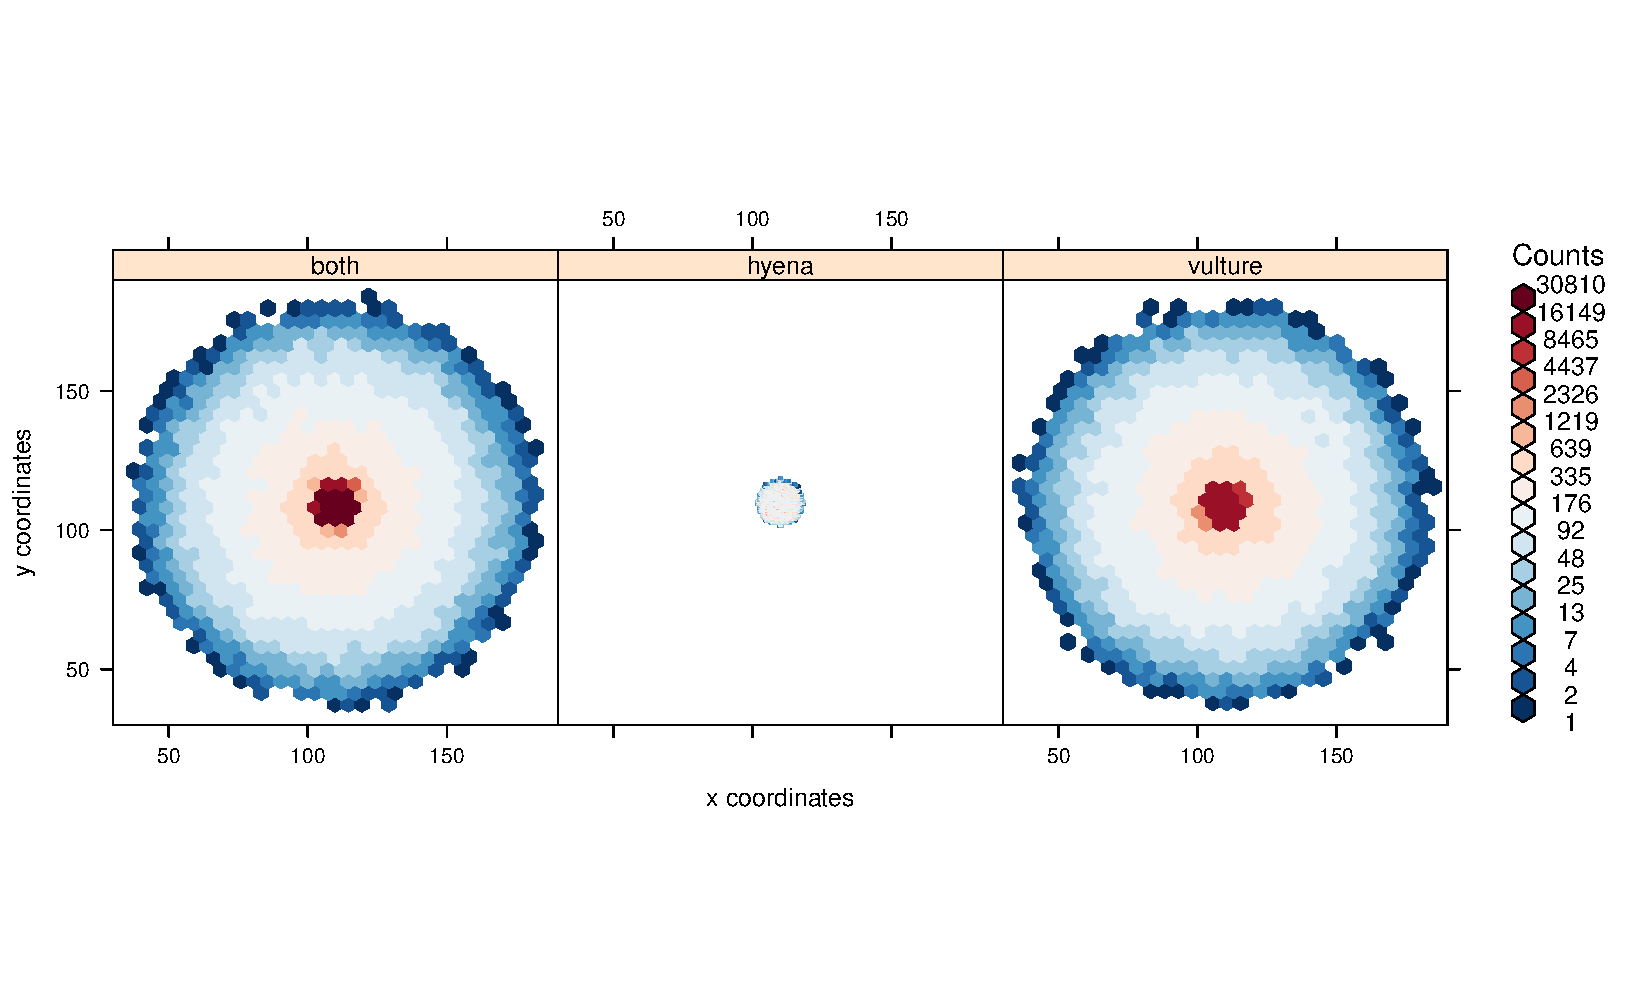
\includegraphics[keepaspectratio,totalheight=0.5\textheight]{nutrientLandscape.pdf}
\caption{Distribution of nutrients throughout the landscape for different scenarios of species compositions. Counts are the raw numbers of nutrients deposited in the each patch}
\label{Nutrient Distributions}
\end{figure}

%---------------------------------------------
%
%       DISCUSSION
%
%---------------------------------------------

\section{Discussion}
Difference in hyenas and vultures. Implications for the future. 

%Biology letters various stuff
\section{Ethics statement}
N/A
\section{Data accessibility statement}
All data and analysis code is available on GitHub (\url{https://github.com/kanead}).
\section{Authors' Contributions}
A.K. and A.J conceived and designed the experiments. A.K. performed the experiments and analysed the data. A.K. and A.J. contributed to the writing of the manuscript. All authors approved the final version of the manuscript.
\section{Competing Interests}
We have no competing interests.
\section{Acknowledgments}
We thank Thomas Guillerme.
\section{Funding statement}
This work was funded by a Trinity College Dublin Teaching Studentship.

\bibliographystyle{vancouver}
\bibliography{References}

%END
\end{document}
